\documentclass{standalone}
\usepackage{tikz}
\usetikzlibrary{positioning, calc}

\begin{document}
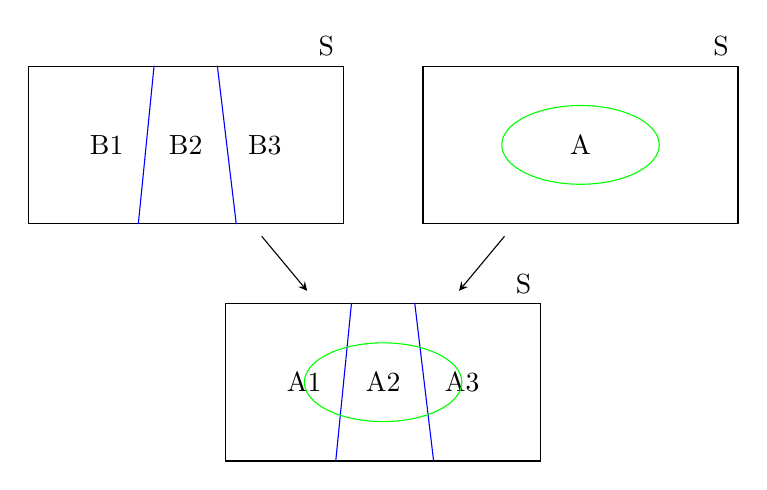
\begin{tikzpicture}
\tikzset{
    myrectangle/.style={
        draw=black,
        minimum width=4cm,
        minimum height=2cm,
    },
    B/.style={
        draw=blue,
    },
    A/.style={
        draw=green,
    },
    >=stealth,
    node distance=1cm and 1cm,
}

    \node[myrectangle] (left) {};
    \node[myrectangle] (right) [right=of left] {};
    \path (left.south east) -- coordinate (tmp) (right.south west);
    \node[myrectangle] (bottom) [below=of tmp] {};

    % "contents" of left node
    \path (left.west) -- node[pos=.25] {B1} (left.east);
    \path (left.west) -- node[pos=.5] {B2} (left.east);
    \path (left.west) -- node[pos=.75] {B3} (left.east);

    \draw[B] ($(left.north west) ! .4 ! (left.north east)$) -- ($(left.south west) ! .35 ! (left.south east)$);
    \draw[B] ($(left.north west) ! .6 ! (left.north east)$) -- ($(left.south west) ! .66 ! (left.south east)$);

    % "contents" of right node
    \draw[A] (right.center) ellipse [x radius=1cm, y radius=.5cm] node {A};

    % "contents" of bottom node
    \path (bottom.west) -- node[pos=.25] {A1} (bottom.east);
    \path (bottom.west) -- node[pos=.5] {A2} (bottom.east);
    \path (bottom.west) -- node[pos=.75] {A3} (bottom.east);

    \draw[B] ($(bottom.north west) ! .4 ! (bottom.north east)$) -- ($(bottom.south west) ! .35 ! (bottom.south east)$);
    \draw[B] ($(bottom.north west) ! .6 ! (bottom.north east)$) -- ($(bottom.south west) ! .66 ! (bottom.south east)$);

    \draw[A] (bottom.center) ellipse [x radius=1cm, y radius=.5cm];

    % arrows
    \begin{scope}[
        shorten >=.2cm,
        shorten <=.2cm,
    ]
        \draw[->, black] (left) -- (bottom);
        \draw[->, black] (right) -- (bottom);
    \end{scope}

    % labels on top
    \node at (left.north east) [anchor=south east] {S};
    \node at (right.north east) [anchor=south east] {S};
    \node at (bottom.north east) [anchor=south east] {S};

\end{tikzpicture}
\end{document}